\everymath{\displaystyle}
\documentclass{beamer}
% \documentclass[handout]{beamer}

%\usepackage[pdftex]{color,graphicx}
\usepackage{amsmath,amssymb,amsfonts}

\mode<presentation>
{
  % \usetheme{Darmstadt}
  % \usetheme[hideothersubsections]{Hannover}
  % \usetheme[hideothersubsections]{Goettingen}
  \usetheme[hideothersubsections, right]{Berkeley}

  \usecolortheme{seahorse}
  % \usecolortheme{dolphin}
  \usecolortheme{rose}
  % \usecolortheme{orchid}

  \useinnertheme[shadow]{rounded}

  \setbeamercovered{transparent}
  % or whatever (possibly just delete it)
}

\mode<handout>{
  \setbeamercolor{background canvas}{bg=black!5}
  \usepackage{pgfpages}
  \pgfpagesuselayout{4 on 1}[a4paper,border shrink=5mm, landscape]
}

\usepackage[brazilian]{babel}
% or whatever

% \usepackage[latin1]{inputenc}
\usepackage[utf8]{inputenc}
% or whatever

\usepackage{times}
%\usepackage[T1]{fontenc}
% Or whatever. Note that the encoding and the font should match. If T1
% does not look nice, try deleting the line with the fontenc.


\title%[] % (optional, use only with long paper titles)
{Tutorial Prático II}

\subtitle
{Correlação e Regressão} % (optional)

\author%[] % (optional, use only with lots of authors)
{Felipe Figueiredo}% \and S.~Another\inst{2}}
% - Use the \inst{?} command only if the authors have different
%   affiliation.

\institute[] % (optional, but mostly needed)
{Instituto Nacional de Traumatologia e Ortopedia
}
  % \inst{1}%
  % Department of Computer Science\\
  % University of Somewhere
  % \and
  % \inst{2}%
  % Department of Theoretical Philosophy\\
  % University of Elsewhere}
% - Use the \inst command only if there are several affiliations.
% - Keep it simple, no one is interested in your street address.

\date%[] % (optional)
{}

% \subject{Talks}
% This is only inserted into the PDF information catalog. Can be left
% out. 



% If you have a file called "university-logo-filename.xxx", where xxx
% is a graphic format that can be processed by latex or pdflatex,
% resp., then you can add a logo as follows:

\pgfdeclareimage[height=1.6cm]{university-logo}{../logo}
\logo{\pgfuseimage{university-logo}}



% Delete this, if you do not want the table of contents to pop up at
% the beginning of each subsection:
\AtBeginSubsection[]
%\AtBeginSection[]
{
  \begin{frame}<beamer>{Sumário}
    \tableofcontents[currentsection,currentsubsection]
  \end{frame}
}


% If you wish to uncover everything in a step-wise fashion, uncomment
% the following command: 

\beamerdefaultoverlayspecification{<+->}


\begin{document}

\begin{frame}
  \titlepage
\end{frame}

\begin{frame}{Sumário}
  \tableofcontents
  % You might wish to add the option [pausesections]
\end{frame}


%% Template
% \section{}

% \subsection{}

% \begin{frame}{}
%   \begin{itemize}
%   \item 
%   \end{itemize}
% \end{frame}

% \begin{frame}
%   \begin{columns}
%     \begin{column}{5cm}
%     \end{column}
%     \begin{column}{5cm}
%     \end{column}
%   \end{columns}
% \end{frame}

% \begin{frame}{}
%   \includegraphics[height=0.4\textheight]{file1}
%   \includegraphics[height=0.4\textheight]{file2}
%   \includegraphics[height=0.4\textheight]{file3}
%   \begin{figure}
%     \caption{}
%   \end{figure}
% \end{frame}

% \begin{frame}{}
%   \begin{definition}
%   \end{definition}
%   \begin{example}
%   \end{example}
%   \begin{block}{Exercício}
%   \end{block}
% \end{frame}

\section{Associação}

\subsection{Dados}

\begin{frame}{Dados}
  \begin{itemize}
  \item Usaremos os dados do exemplo da aula de correlação (Motulsky, 1995)
  \item Objetivo: refazer as análises do autor no BioEstat
  \end{itemize}
\end{frame}


\begin{frame}{Dados}
  \begin{center}
    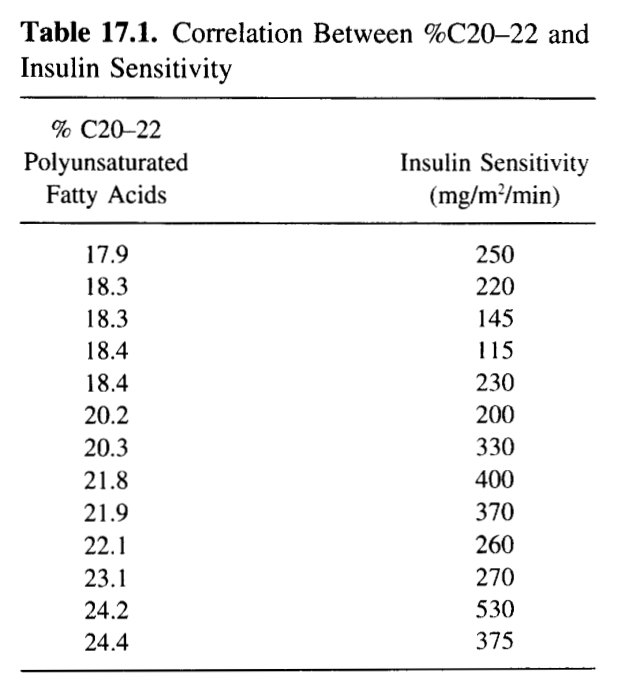
\includegraphics[height=0.9\textheight]{table}
  \end{center}
\end{frame}

\begin{frame}{Dados}
  \begin{center}
    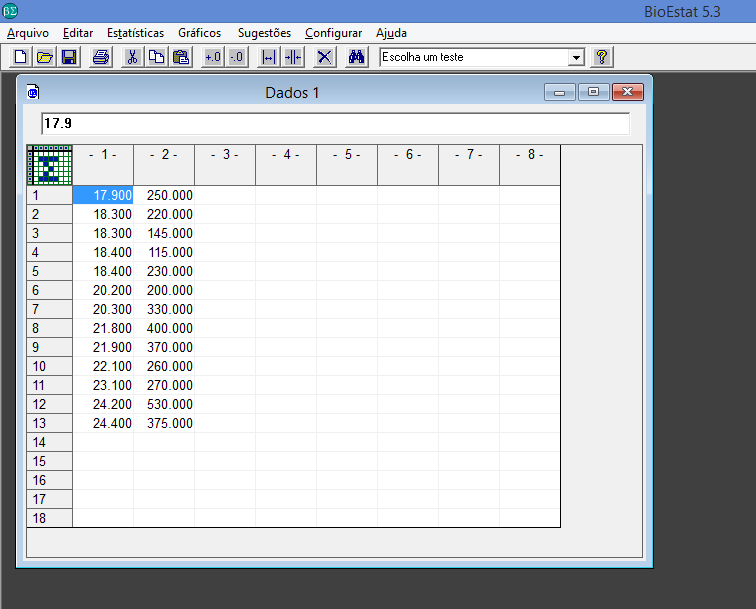
\includegraphics[height=0.9\textheight]{dados}
  \end{center}
\end{frame}


\subsection{Gráfico de Dispersão}

\begin{frame}{Gráfico de Dispersão}
  \begin{center}
    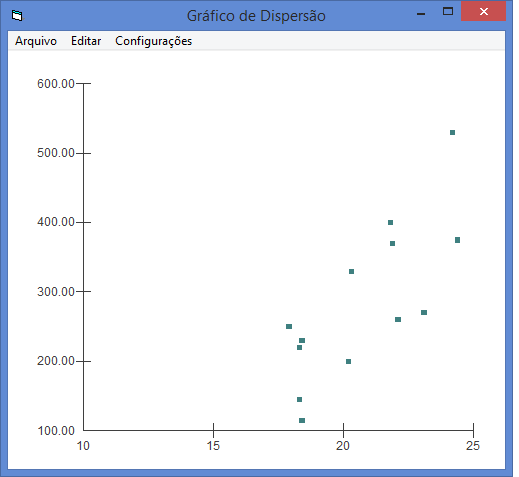
\includegraphics[height=0.9\textheight]{grafico_dispersao}
  \end{center}
\end{frame}


\subsection{Sugestão}

\begin{frame}{Sugestão do BioEstat}
  \begin{center}
    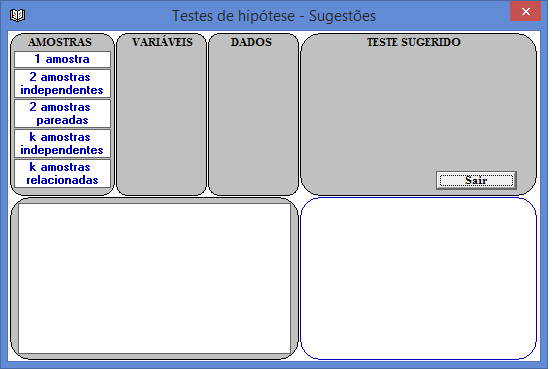
\includegraphics[height=0.9\textheight]{sugestao1}
  \end{center}
\end{frame}

\begin{frame}{Sugestão do BioEstat}
  \begin{center}
    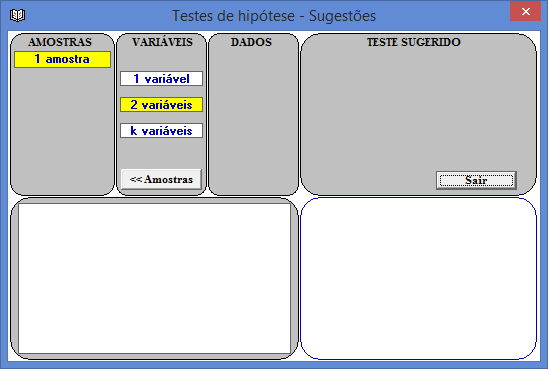
\includegraphics[height=0.9\textheight]{sugestao2}
  \end{center}
\end{frame}

\begin{frame}{Sugestão do BioEstat}
  \begin{center}
    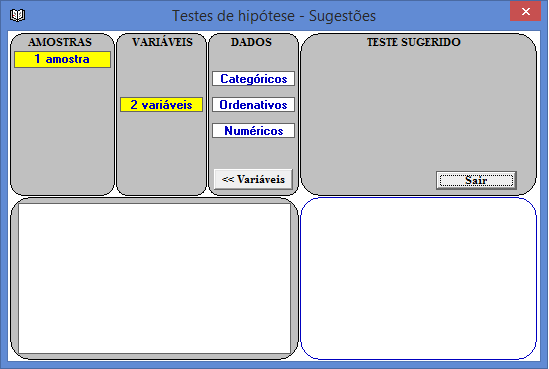
\includegraphics[height=0.9\textheight]{sugestao3}
  \end{center}
\end{frame}

\begin{frame}{Sugestão do BioEstat}
  \begin{center}
    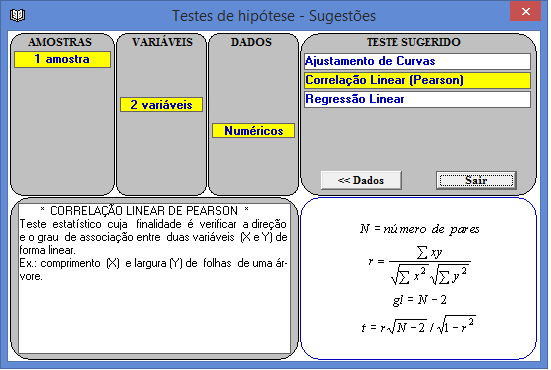
\includegraphics[height=0.9\textheight]{sugestao4}
  \end{center}
\end{frame}

\subsection{Correlação}

\begin{frame}{Correlação}
  \begin{center}
    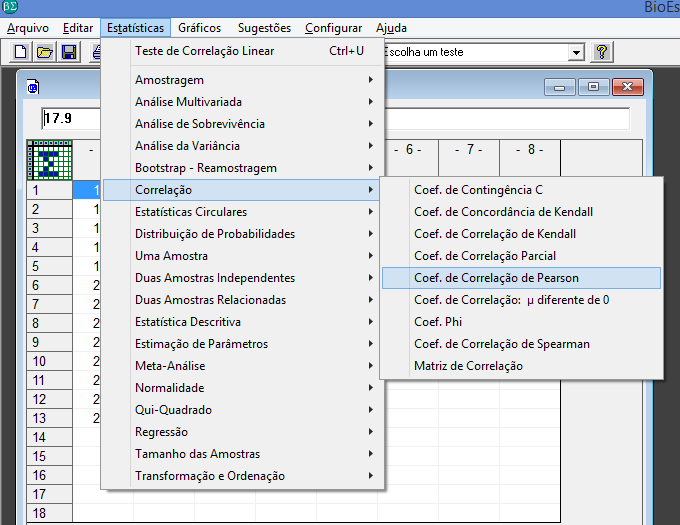
\includegraphics[height=0.9\textheight]{selecao_correlacao}
  \end{center}
\end{frame}

\begin{frame}{Correlação}
  \begin{center}
    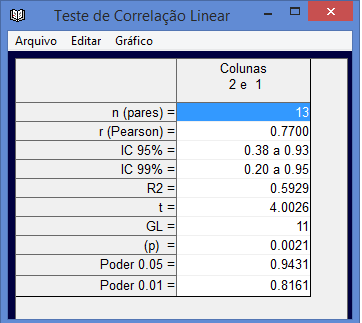
\includegraphics[height=0.9\textheight]{resultado_correlacao}
  \end{center}
\end{frame}


\subsection{Regressão}

\begin{frame}{Regressão}
  \begin{center}
    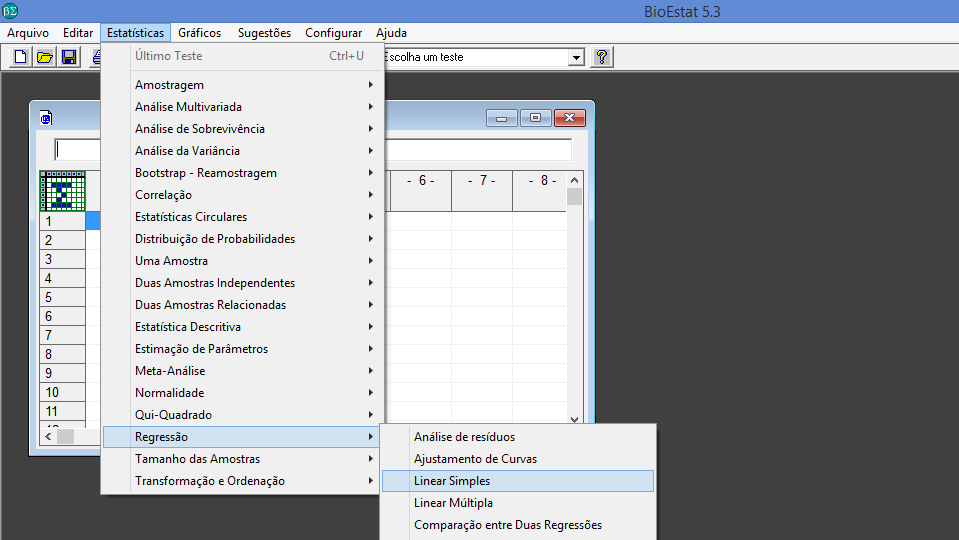
\includegraphics[width=0.9\textwidth]{selecao_regressao}
  \end{center}
\end{frame}

\begin{frame}{Regressão}
  \begin{center}
    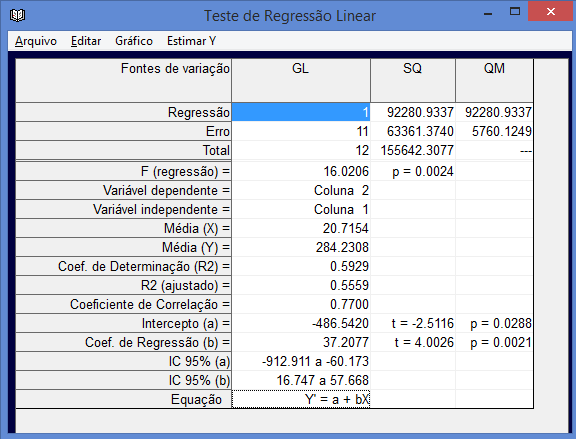
\includegraphics[height=0.7\textheight]{resultado_regressao}
  \end{center}

Selecionar ``Gráfico'' para visualizar a reta regressora
\end{frame}

\begin{frame}{Regressão}
  \begin{center}
    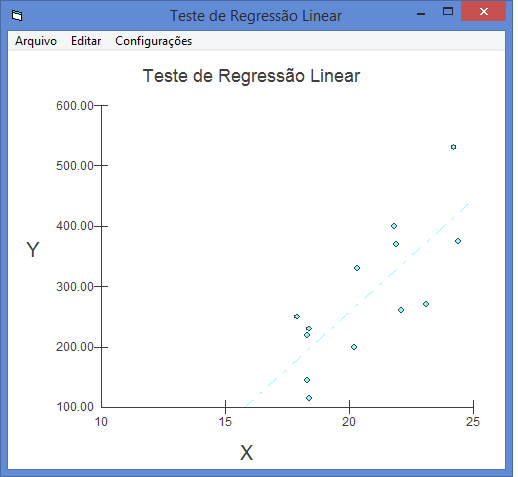
\includegraphics[height=0.9\textheight]{grafico_regressao}
  \end{center}
\end{frame}

\begin{frame}{Interpolação}
  \begin{itemize}
  \item Agora que temos o modelo, podemos fazer estimativas
    para regiões onde não há dados!
  \item Basta selecionar ``Estimar Y'' e estipular um valor de $X$
  \end{itemize}
\end{frame}

\begin{frame}{Regressão}
  \begin{center}
    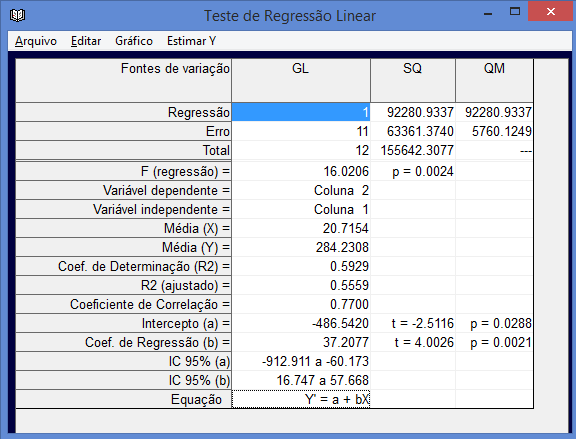
\includegraphics[height=0.7\textheight]{resultado_regressao}
  \end{center}

Selecionar ``Estimar Y'' e estipular um valor de $X$
\end{frame}

\begin{frame}{Dados}
  \begin{center}
    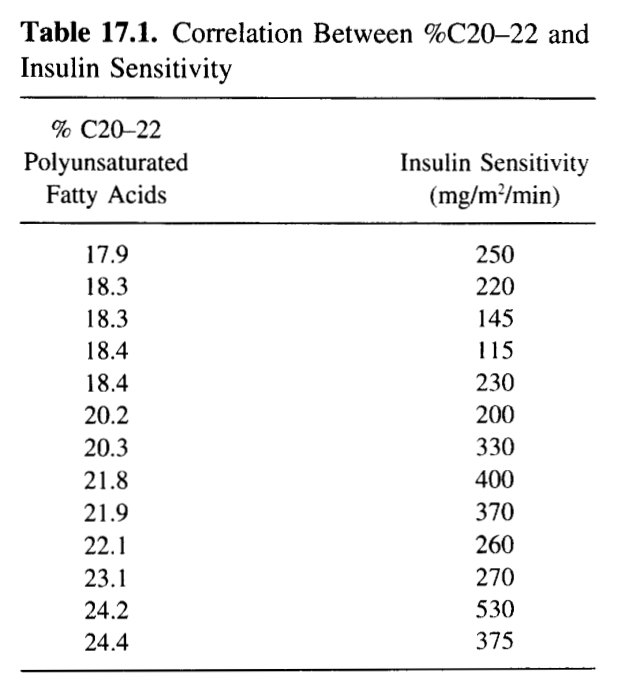
\includegraphics[height=0.7\textheight]{table}

    Qual seria o índice de insulina esperado, se $X=19.5$?
  \end{center}
\end{frame}


\begin{frame}{Interpolação}
  \begin{center}
    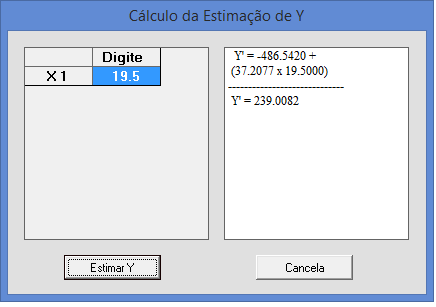
\includegraphics[height=0.9\textheight]{interpolacao}
  \end{center}
\end{frame}


\end{document}
